% Section 2 - Core library
% Roberto Masocco <roberto.masocco@uniroma2.it>
% Alessandro Tenaglia <alessandro.tenaglia@uniroma2.it>
% June 5, 2024

% ### Core library ###
\section{Core library}
\graphicspath{{figs/section2/}}

% --- Code organisation ---
\begin{frame}{Code organisation}
	One of the main features of the MARTe2 architecture is the \textbg{decoupling} of:
	\begin{itemize}
		\item the platform \textbg{architecture}, \emph{i.e.}, \texttt{x86}, \texttt{armv8}...
		\item the \textbg{environment} details, \emph{i.e.}, Linux, FreeRTOS, Windows;
		\item the \textbg{real-time algorithms}, \emph{i.e.}, the user code.
	\end{itemize}
\end{frame}
\begin{frame}{Code organisation}
	\begin{figure}
		\centering
		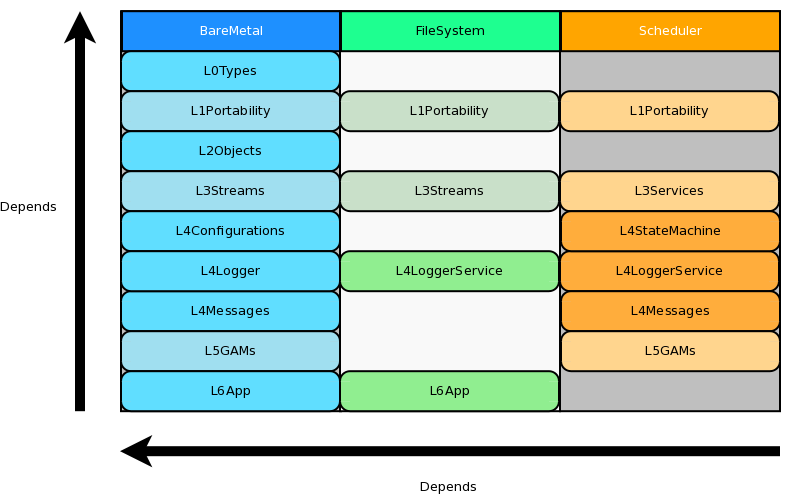
\includegraphics[scale=.35]{Tiers.png}
		\label{fig:tiers}
		\caption{Core libraries organization.}
	\end{figure}
\end{frame}
\begin{frame}{Code organisation}
	The official source code is divided into the following \textbg{two public repositories}:
  \begin{itemize}
    \item \href{https://vcis-gitlab.f4e.europa.eu/aneto/MARTe2}{\color{blue}\underline{\textbf{MARTe2}}}: the core library.
    \item \href{https://vcis-gitlab.f4e.europa.eu/aneto/MARTe2-components}{\color{blue}\underline{\textbf{MARTe2-components}}}: additional software modules to extend the core library.
  \end{itemize}
\end{frame}

% --- Makefile ---
\begin{frame}{Makefile}
	\begin{columns}
		\column{.5\textwidth}
		The build of the core library, as well as any MARTe2 project, follows this structure:
		\begin{enumerate}
			\item The \texttt{Makefile.os-arch} defines the \textbg{TARGET} operating system and architecture.
			\item The \texttt{Makefile.inc} defines all the common rules.
			\item The \texttt{MakeDefaults} defines the specific rules for the \textbg{TARGET}.
		\end{enumerate}
		\column{.5\textwidth}
		\begin{figure}
			\centering
			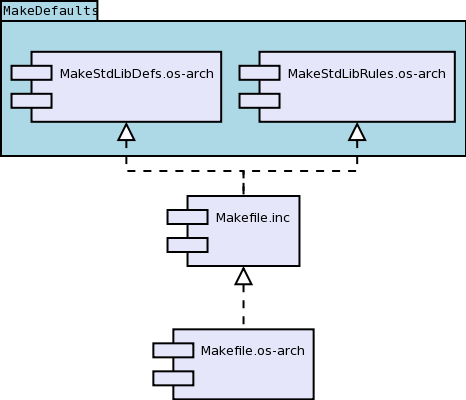
\includegraphics[scale=.4]{Makefiles.png}
			\label{fig:makefiles}
			\caption{Makefile structure (bottom to top).}
		\end{figure}
	\end{columns}
\end{frame}
